\documentclass[9pt, t]{beamer}
\usefonttheme{serif}
\usecolortheme[named=black]{structure}
\setbeamertemplate{footline}[frame number]{}
\setbeamertemplate{navigation symbols}{}

\usepackage[normalem]{ulem} % underlining
\setlength{\parskip}{0.5em}
\usepackage{tabto}
% LANGUAGE + FONT
		    
\usepackage[english]{babel}

\usepackage{natbib}
\bibpunct[: ]{[}{]}{;}{a}{}{,}
\bibliographystyle{plainnat}

\usepackage{fontspec}  
\setmainfont{Fira Sans}


% DRAWING

\usepackage{tikz}
\usepackage{tikz-qtree}
\usetikzlibrary{shapes.geometric}
\usetikzlibrary{trees,arrows}
\usetikzlibrary{positioning}

% LINGUISTICS 

\usepackage{expex}
\lingset{aboveglftskip=-1ex, belowglpreambleskip=0ex, belowexskip=1ex, aboveexskip=1ex, interpartskip=0ex}

\gathertags
\usepackage[glossaries]{leipzig}
% \makeglossaries

\usepackage{stmaryrd}

\usepackage[linguistics]{forest}
    
% MATH
\usepackage{amssymb}

\graphicspath{{images/}}

\AtBeginSection[]{
    \begin{frame}
        \frametitle{TOC}
            \tableofcontents[currentsection]
    \end{frame}
}
    
\resetcountonoverlays{excnt}

\title{Latvian classifying adjectives}
\author{Arkady Shaldov}
\institute{HSE Moscow, Laboratory on formal models in linguistics}

\date{Bucharest definiteness workshop, 08.12.2023}


% -------------------------- текстиктекстиктекстик --------------------------
\begin{document}

\NumTabs{14}

\begin{frame}
    \titlepage
    
\end{frame}

\begin{frame}
    \frametitle{Intro}

    Latvian definite adjectival suffix is required on classifying adjectives

    \pex<>
        \a \begingl
            \gla skaist-s lācis//
            \glb beautiful-\Nom{} bear//
            \glft 'a beautiful bear'//
        \endgl
        \a \begingl
            \gla skaist-ai-s lācis//
            \glb beautiful-\Def{}-\Nom{} bear//
            \glft 'the beautiful bear'//
        \endgl
        \a \begingl
            \gla balt-ai-s lācis//
            \glb white-\Def{}-\Nom{} bear//
            \glft 'a / the polar bear'//
        \endgl
    \xe

\end{frame}

\section{Kinds and definiteness}
\begin{frame}
    \frametitle{On kinds}

    Total (intensional) individuals for which a predicate is true \citep{chierchia1998}

    \pex<>
        \a Dogs\tab\tab cannot\tab\tab purr\tab\tab / \tab are widespread.
        \a I$_{\Def}$ cani\tab non possono\tab fare le fusa / \tab sono diffusi.
        \a Собаки\tab не умеют\tab\tab мурчать\tab / \tab распространены.
    \xe

    Singular expressions can sometimes be used

    \pex<kind>
        \a The dodo\tab is extinct.
        \a Il$_{\Def}$ dodo\tab è estinto.\trailingcitation{\citep{chierchia1998}}
        \a Додо\tab\tab вымер.
    \xe

    But only for \textit{well-established kinds} \citep{carlson1977,dayal2004}: an asymmetry
    
    \pex<notkind>
        \a \ljudge{*} The tiger with gray stripes is extinct.
        \a \ljudge{\textsuperscript{OK}} Tigers with gray stripes are extinct.
    \xe

\end{frame}

\begin{frame}
    \frametitle{\citep{chierchia1998}}

    \textsc{down} operator $^\cap$ turns an intensional predicate $\langle s, \langle e,t\rangle\rangle$ to the maximal intensional individual $\langle s, e\rangle$
    \ex<kinddef>
        For any property P

        $^\cap P_{\langle s,\langle e,t\rangle\rangle} = \lambda s.\iota P_s \text{ iff }\lambda s.\iota P_s\in K$
    \xe

    Symmetrical \textsc{up} operator $^\cup$

    \ex<>
        $^\cup k = \lambda x.\ x\le k_s$
    \xe

    DKP

    \ex<dkp>
        If P applies to objects and k denotes a kind, then\\
        $P(k) = \exists x[^\cup k(x) \land P(x)]$
    \xe
\end{frame}

% \begin{frame}
%     \frametitle{Виды и определенность}

%     \pex<kinddef>
%         \a $^\cap P_{\langle s\langle e,t\rangle\rangle} = \lambda s.\iota P_s\text{ iff }\iota P_s \in K$

%         \a $\iota P = \begin{cases}
%             x & P(x)\land\forall y[y\not\le x](\neg P(x))\\
%             \text{неопределено} & \text{в противном случае}
%         \end{cases}$
%     \xe

%     \pause
%     Оператор понижения отличается от йота-оператора только интенсиональностью и ограничением $\in K$
    
%     Итальянский \citep{chierchia1998}: интенсионализирующий оператор $^\land$ с йота-оператором
    
%     \ex<>
%         \begingl
%             \gla I cani sono diffusi.//
%             \glb \Def{} собаки \Cop.\Pl{} распространены//
%             \glft 'Собаки распространены.'//
%         \endgl
%     \xe

% \end{frame}
\begin{frame}
    \frametitle{Singulars as kinds}

    
    \ex<>
    The African lion is extinct.
    \xe
    
    \citep{krifka1999,dayal2004}: it is not just \textit{the}
    
    
    \pex<>
        \a Every / a / one (kind of) lion is extinct.\trailingcitation{\citep{dayal2004}}
        \a Two / three / most (kinds of) lions are extinct.
        \a $\llbracket \textsc{lion} \rrbracket = \{\textsc{african lion, asian lion, berber lion}\}$
    \xe
                
    Nouns are ambiguous between properties of objects and kinds

    Determiners combine with properties of kinds just the same

\end{frame}

\section{The data}
\begin{frame}
    \frametitle{Definiteness}
    
    In Latvian, definiteness is marked with suffix \textit{-ai-} on adjectives\footnote{and is unmarked when there is no adjective}

    \pex<def>
        \a \begingl
            \gla lācis//
            \glb bear//
            \glft 'a / the bear'//
        \endgl
        \a \begingl
            \gla skaist-s lācis//
            \glb beautiful-\Nom{} bear//
            \glft 'a beautiful bear'//
        \endgl
        \a \begingl
            \gla skaist-ai-s lācis//
            \glb beautiful-\Def{}-\Nom{} bear//
            \glft 'the beautiful bear'//
        \endgl
    \xe

\end{frame}

\begin{frame}
    \frametitle{Paradigm [Kalnaca, Lokmane 2021]}

    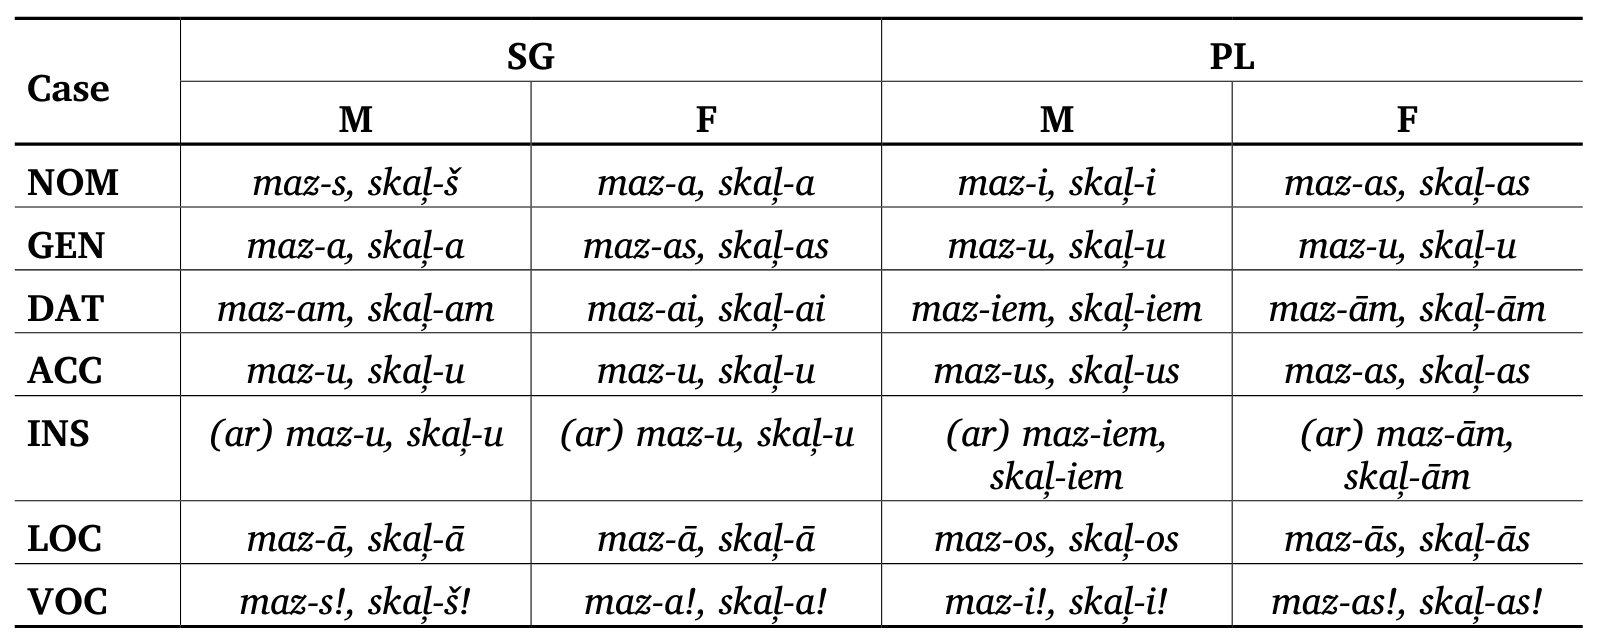
\includegraphics[width=30em]{lat paradigm 1.png}
    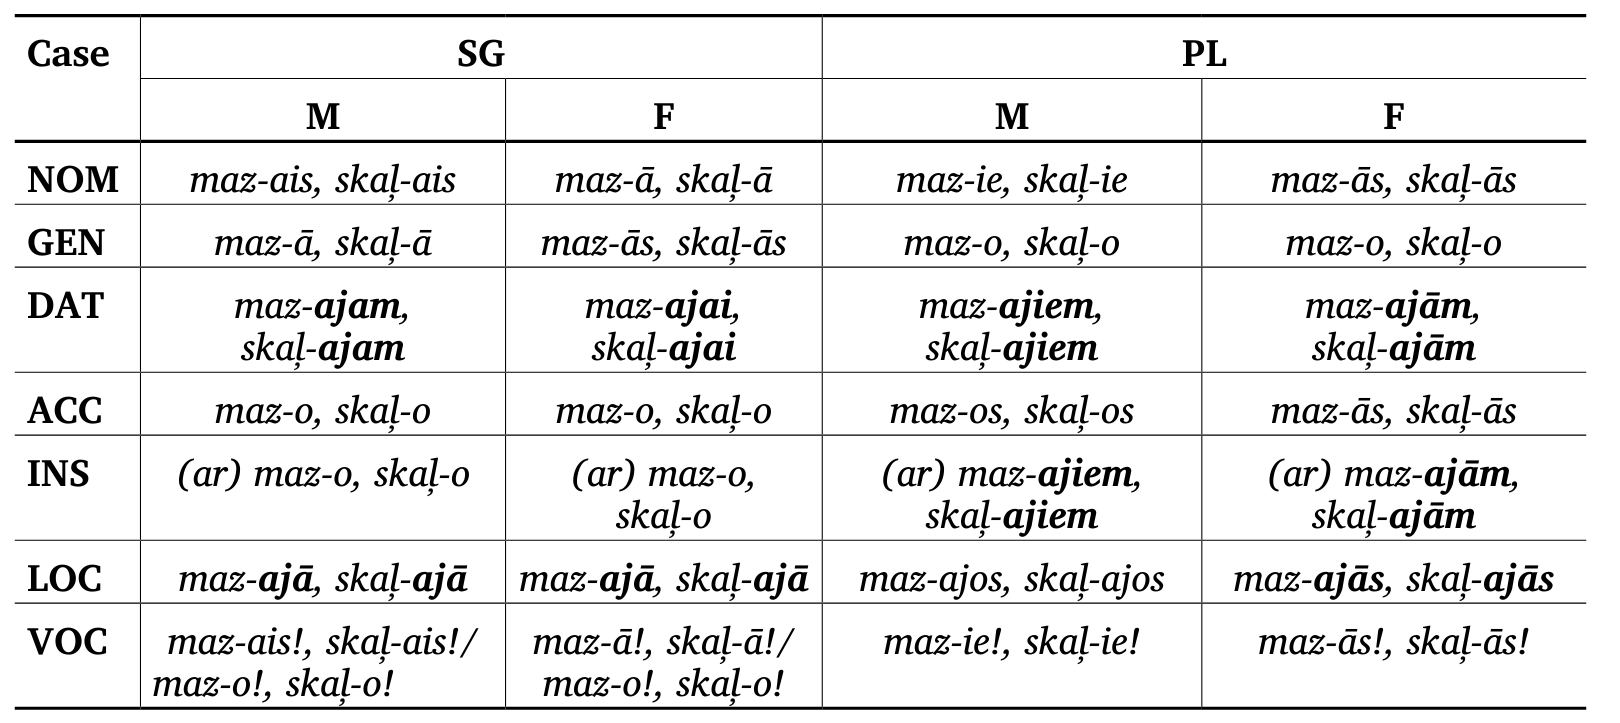
\includegraphics[width=30em]{lat paradigm 2.png}

\end{frame}

\begin{frame}
    \frametitle{Classifying adjectives}

    The same marker is required on classifying adjectives --- those that denote established concepts

    \pex<class>
        \a \begingl
            \gla formālā\ /\ *-a loģika//
            \glb formal-\Def{}.\F.\Nom{}\ /\ -\F.\Nom{} logics//
            \glft 'formal logics'//
        \endgl
        \a \begingl
            \gla balt-*(ai)-s lācis//
            \glb white-\Def{}-\Nom{} bear//
            \glft 'a / the polar bear'//
        \endgl
    \xe
    
    \pause
    Independent of the proper definiteness marker
    
    \pex<>
        \a \begingl
            \gla skaist-s balta-ai-s lācis//
            \glb beautiful-\Nom{} white-\Def{}-\Nom{} bear//
            \glft 'a beautiful polar bear'//
        \endgl
        \a \begingl
            \gla skaist-ai-s balta-ai-s lācis//
            \glb beautiful-\Def-\Nom{} white-\Def{}-\Nom{} bear//
            \glft 'a beautiful polar bear'//
        \endgl
    \xe

\end{frame}

\begin{frame}
    \frametitle{Independent of number}

    Applies to plurals and masses as well

    \pex<>
        \a<> \begingl
            \gla balt-ai-s lācis//
            \glb white-\Def{}-\Nom{} bear//
            \glft 'a / the polar bear'//
        \endgl
        \a<> \begingl
            \gla balt-ie lāči//
            \glb white-\Def{}.\Pl.\Nom{} bear//
            \glft '(the) polar bears'//
        \endgl
        \a \begingl
            \gla balt-ā tēja//
            \glb white-\Def.\F.\Nom{} tea//
            \glft '(the) white tea'//
        \endgl
    \xe

\end{frame}

\begin{frame}
    \frametitle{NP-internal}

    \citep[etc.]{rutpro2006}: classifying adjectives are generated NP-internally (cf. \textit{termininological units})

    E.g. linear adjacency

    \pex<lin>
        \a \begingl
            \gla balt-ai-s liel-ai-s skudrlācis//
            \glb white-\Def{}-\Nom{} big-\Def-\Nom{} anteater//
            \glft 'the white giant anteater'//
        \endgl
        \a \begingl
            \gla\ljudge{\#}liel-ai-s balt-ai-s skudrlācis//
            \glb big-\Def-\Nom{} white-\Def{}-\Nom{} anteater//
            \glft 'the white giant anteater'//
        \endgl
    \xe

\end{frame}

\begin{frame}
    \frametitle{A property of NP-internal adjectives?}

    Passive participles (having larger structure, e.g. \textit{viegli gāzēts} 'lightly sparkling') are not objects to the marking

    Too large to fit inside NP?

    \pex<ptcp>
        \a<> \begingl
            \gla dzēram-ai-s ūdens//
            \glb drinking-\Def-\Nom{} water//
            \glft 'drinking water'//
        \endgl
        \a<> \begingl
            \gla gāzē-t-(\#ai)-s ūdens//
            \glb aerate-\Ptcp-\Def-\Nom{} water//
            \glft 'sparkling water'//
        \endgl
    \xe

    Not morphology, cf.

    \ex<>
        \begingl
            \gla ģimenē lieto-t-ā valoda//
            \glb in\_family use-\Ptcp-\Def.\F.\Nom{} language//
            \glft 'the language used in family'//
        \endgl
    \xe

\end{frame}

\begin{frame}
    \frametitle{Well-establishedness}

    The concept referred by the adj+n complex must be contextually salient

    \pex<disc>
        \a<cmn> \begingl
            \gla šodien uz ielas atradu elektrisk-o (*-u) tējkann-u//
            \glb today on street found electric-\M.\Def.\Acc{} (\Acc{}) kettle-\Acc{}//
            \glft 'Today I found an electric kettle in the street.'//
        \endgl
        \a<uncmn> \begingl
            \gla šodien uz ielas atradu elektrisk-u (*-o) zirnekl-i//
            \glb today on street found electric-\M.\Acc{} (\Def.\Acc) spider-\Acc{}//
            \glft 'Today I found an electric spider in the street.'//
        \endgl
    \xe

    \pause

    Latvian kind-referring \textit{-ai-} has similar distribution to English kind-referring singular \textit{the}

    Except that it doesn't require the whole DP to refer to a kind

    And is low (below number)

\end{frame}

\section{Earlier approaches}
\begin{frame}
    \frametitle{\citep{rutpro2006}, Lithuanian}

    A reflex of the adjective movement to some ClasP

    \begin{itemize}
        \item Barely accounts for polysemy with definiteness
    \end{itemize}

\end{frame}

\begin{frame}
    \frametitle{\citep{sereikaite2017}, Lithuanian}

    A $^\cap$ above every NP.

    \ex<>
        \begingl
            \gla gražus-is baltas-is lokys//
            \glb beautiful-\Def{} white-\Def{} bear//
            \glft 'beautiful polar bear'\trailingcitation{Lithuanian}//
        \endgl
    \xe
    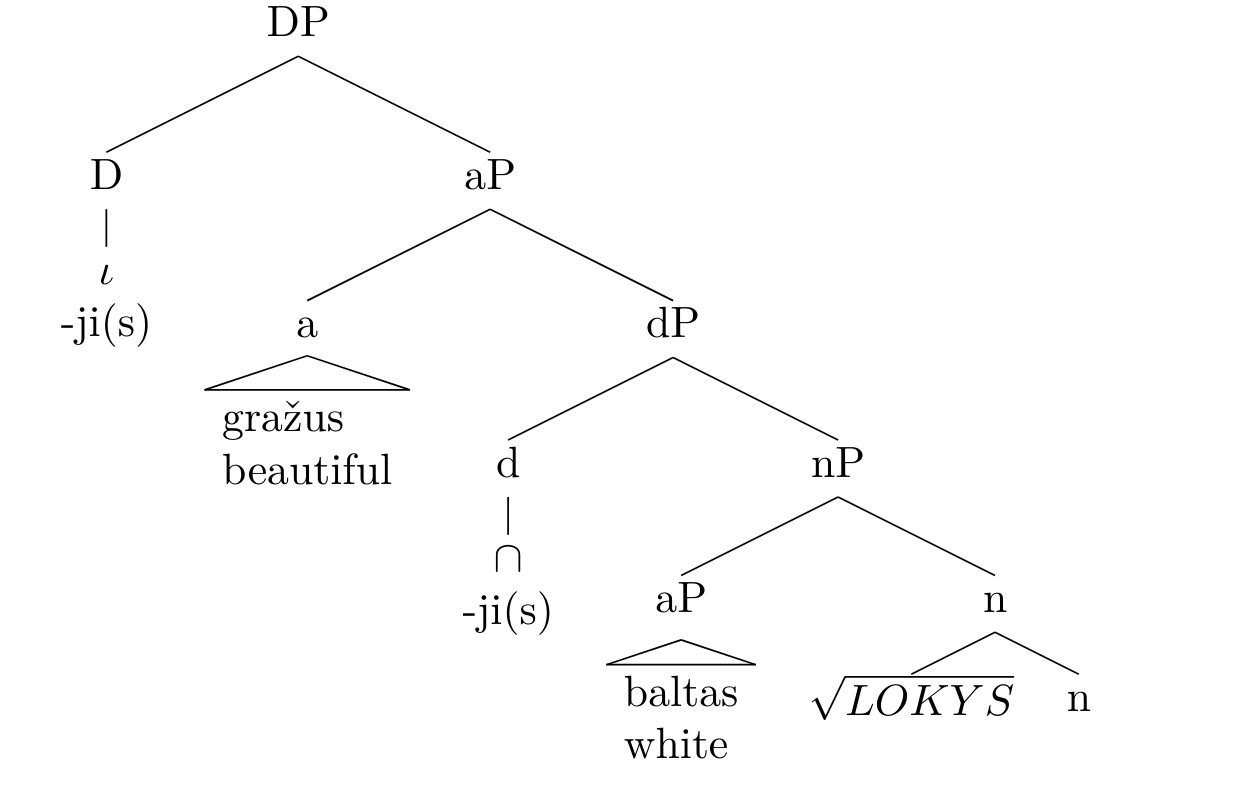
\includegraphics[width=20em]{sereitree.png}

    \pause
    \begin{itemize}
        \item dP of type $e$: A $^\cup$ is also required between dP and aP (more ad hoc projections)
    \end{itemize}

\end{frame}

\section{The proposal}
\begin{frame}
    \frametitle{Partitive specificity}

    \begin{itemize}
        \item Latvian is an articless language like Russian and Hindi \citep{dayal2004}
        \item \textit{-ai-} marks partitive specificity, not definiteness \citep{enc1991}
        \item It is visible when the definite adjective is below an indefinite
    \end{itemize}
      
    \pex<>
        \a \begingl
            \gla liel-ai-s balt-ai-s kaķis//
            \glb big-\Def-\Nom{} white-\Def-\Nom{} cat//
            \glft 'the big white cat'//
        \endgl
        \a \begingl
            \glpreamble \{Walking down the street, I saw several white cats.\}//
            \gla liel-s balt-ai-s kaķis//
            \glb big-\Nom{} white-\Def-\Nom{} cat//
            \glft 'a big white cat \{approached me and began to meow.\}'//
        \endgl
    \xe

    \ex<>
        \begingl
            \glpreamble \{There are several cups on the table, both big and small. I ask:\}//
            \gla iedod man kād-u liel-o krūzi//
            \glb give me some-\Acc{} big-\Def{}.\Acc{} cup-\Acc{}//
            \glft 'Give me one of the big cups.'//
        \endgl
    \xe

\end{frame}

\begin{frame}[c]
    \frametitle{Partitive specificity}

    \begin{itemize}
        \item \textit{-ai-} marks partitive specificity, not definiteness
    \end{itemize}

    \ex<>
        $\llbracket ai \rrbracket = \lambda P\lambda x.\ x\le \iota P$
    \xe

    \pause
    
    \ex<>
        \begingl
            \gla balt-ai-s kaķis//
            \glb white-\Def-\Nom{} cat//
            \glft $\lambda y.\ y\le\iota(\lambda x.\ \textsc{white}(x) \land \textsc{cat}(x))$\\
            True for any individual in the plurality of contextually salient white cats//
        \endgl
    \xe

    Ignoring intensionality, $\llbracket ai \rrbracket (P) = ^{\cup}(^{\cap} P)$


\end{frame}

\begin{frame}
    \frametitle{Now to kinds}

    \begin{itemize}
        \item All Latvian nouns are unambiguously taxonomic in the sense of \citep{dayal2004}
        \item They are turned object-referring by the first \textit{-ai-} they combine with        
    \end{itemize}
    
    \ex 
        $\llbracket ai \rrbracket (\textsc{polar bear}) = \lambda x. x\le \iota \textsc{polar bear} = \lambda x. x\text{ is a polar bear}$
    \xe

    \begin{itemize}
        \item The definiteness requirement is satisfied if the kind is well-established (i.e. salient)
    \end{itemize}
    

\end{frame}

\begin{frame}
    \frametitle{Definiteness and kinds}

    \pex
        \a<>\begingl
            \gla liel-s \ljudge{[$_\text{AP}$\ }balt-ai-s @ kaķis\judge{]}//
            \glb big-\Nom{} white-\Def-\Nom{} cat//
            \glb $\lambda x.\ \textsc{big}(x)$ $\lambda x.\ x\le\iota(\lambda x.\ \textsc{white}(x)$ $\ \land\ \textsc{cat}(x))$//
            \glft 'An indefinite big individual in the plurality of contextually salient white cats.'\vspace{1em}//
        \endgl
        \a<> \begingl
            \gla liel-s \ljudge{[$_\text{NP}$\ }balt-ai-s @ lācis\judge{]}//
            \glb big-\Nom{} white-\Def-\Nom{} bear//
            \glb $\lambda x.\ \textsc{big}(x)$ $\lambda x.\ x\le\iota(\lambda x.\ \textsc{white\_}$ $\textsc{bear}(x))$//
            \glft 'An indefinite big individual in the plurality of polar bears (a contextually salient kind).'//
        \endgl
    \xe
\end{frame}

\begin{frame}
    \frametitle{Maximize}

    Why can't a definite adjective be above an indefinite one?

    \ex<>
        \begingl
            \gla liel-ai-s balt-*(ai)-s kaķis//
            \glb big-\Def-\Nom{} white-\Def-\Nom{} cat//
            \glft 'the big white cat'//
        \endgl
    \xe

    \pause
    
    A case of Maximize presupposition \citep{heim1991, copbeav2015}
    \begin{itemize}
        \item[] A plurality of salient cats exists
        \item[$\Rightarrow$] A plurality of salient white cats exists
        \item[$\Rightarrow$] The presupposition on \textit{baltais} is always satisfied
    \end{itemize}

\end{frame}

\begin{frame}
    \frametitle{Bare nouns?}

    Partitive interpretation is unavailable for high \textit{-ai-}

    \pex<bare>
        \a<clas> \begingl
            \gla balt-ai-s lācis//
            \glb white-\Def{}-\Nom{} bear//
            \glft 'a / the polar bear'//
        \endgl
        \a<attr> \begingl
            \gla skaist-ai-s lācis//
            \glb beautiful-\Def{}-\Nom{} bear//
            \glft '\#one of the beautiful bears'//
        \endgl
    \xe

    \pause
    \begin{itemize}
        \item Only $\iota $ and $^\cap$ available as a type-shifters 
        \item[$\Rightarrow$] Only maximal individual in (\getfullref{bare.attr})
        \item[$\Rightarrow$] $^\cap$ can be applied to (\getfullref{bare.clas}), and then DKP \citep{chierchia1998}
    \end{itemize}


\end{frame}

\begin{frame}
    \frametitle{Summary}

    \begin{itemize}
        \item There is a definiteness marker above any NP in Latvian
        \item Monosemy can be derived if we assume the marker marks partitive specificity
        \item The specificity, thus, is specificity of a taxonomic individual
        \item Requires an assumption that all Latvian nouns are inherently taxonomic
        \end{itemize}

\end{frame}

\begin{frame}
    \frametitle{Sources}

    {\footnotesize \bibliography{ref.bib}}

\end{frame}
\end{document}
